\section{Real-time analysis}
\label{rta}
The issue of having to process large quantities of data in very short time periods is common to both HEP and industry, and remains a persistent problem in expansion of both areas. \cite{hu-big-data}\par
Real-time analysis is an umbrella term for a collection of techniques in data processing wherein data is processed in real-time, i.e. between recording and storage, often referred to as being ``online''.

\subsection{Principles of RTA}%A problem common to HEP and industry}
\label{common-problem}
In HEP, this is commonly seen in trigger systems, for example the LHCb trigger shown diagrammatically in Figure~\ref{lhcb-trigger}. Since it is not possible to record the detector output and carry out event reconstruction at the LHC collision rate of {40}{MHz}, a trigger must be devised to select only those events which are relevant to the physics goals of a given experiment. Such a trigger conventionally consists of a hardware trigger acting directly on parts of the detector output, and a staged software trigger, applying gradually more fine-tuned selections with increasing amounts of reconstructed event detail.\par
\begin{figure*}
    \centering
    % Use the relevant command for your figure-insertion program
    % to insert the figure file. See example above.
    % If not, use
    \vspace*{5cm}       % Give the correct figure height in cm
    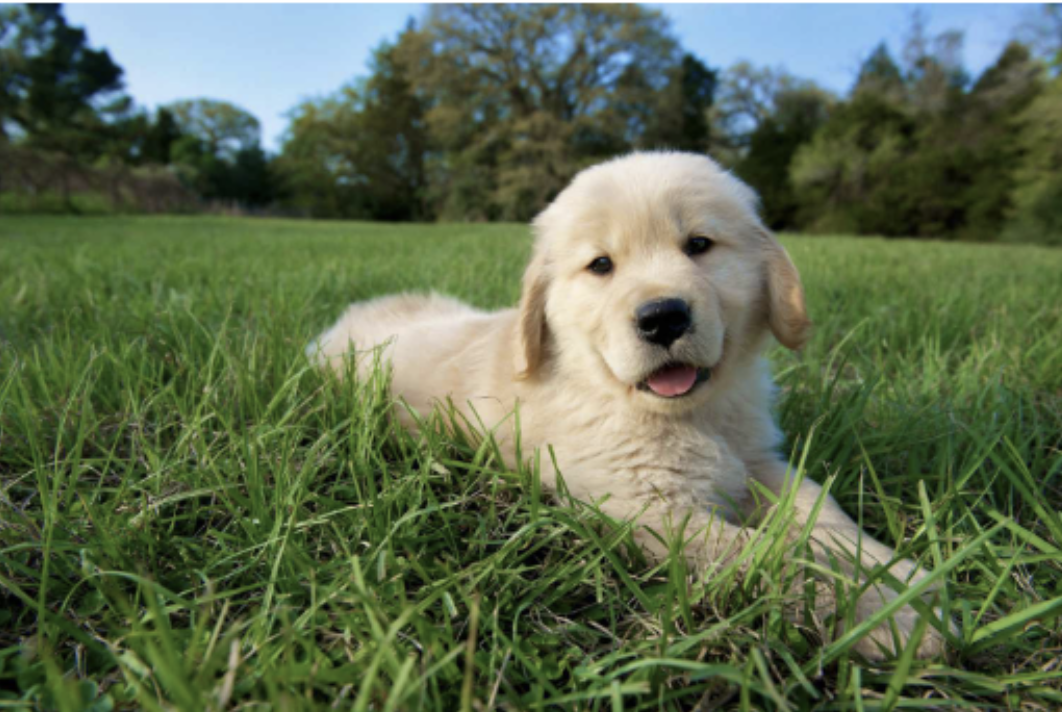
\includegraphics[width=7cm,clip]{/Users/jgooding/Documents/SMARTHEP/CHEP2023/CHEP2023/proceedings/figures/placeholder.png}
    \caption{Trigger framework of the LHCb Experiment during Run 3 of the LHC. In Run 3, LHCb operates an entirely software-based trigger, processing events at the collision rate of {40}{MHz}. Additionally, calibration of the detector is carried out in real time.}
    \label{lhcb-trigger}       % Give a unique label
\end{figure*}
In industry, the limitations of the scale of ``big data'' looms over many applications of computing. However, \par
It is therefore ... Figure~\ref{rta-diagram}
\begin{figure*}
    \centering
    % Use the relevant command for your figure-insertion program
    % to insert the figure file. See example above.
    % If not, use
    \vspace*{5cm}       % Give the correct figure height in cm
    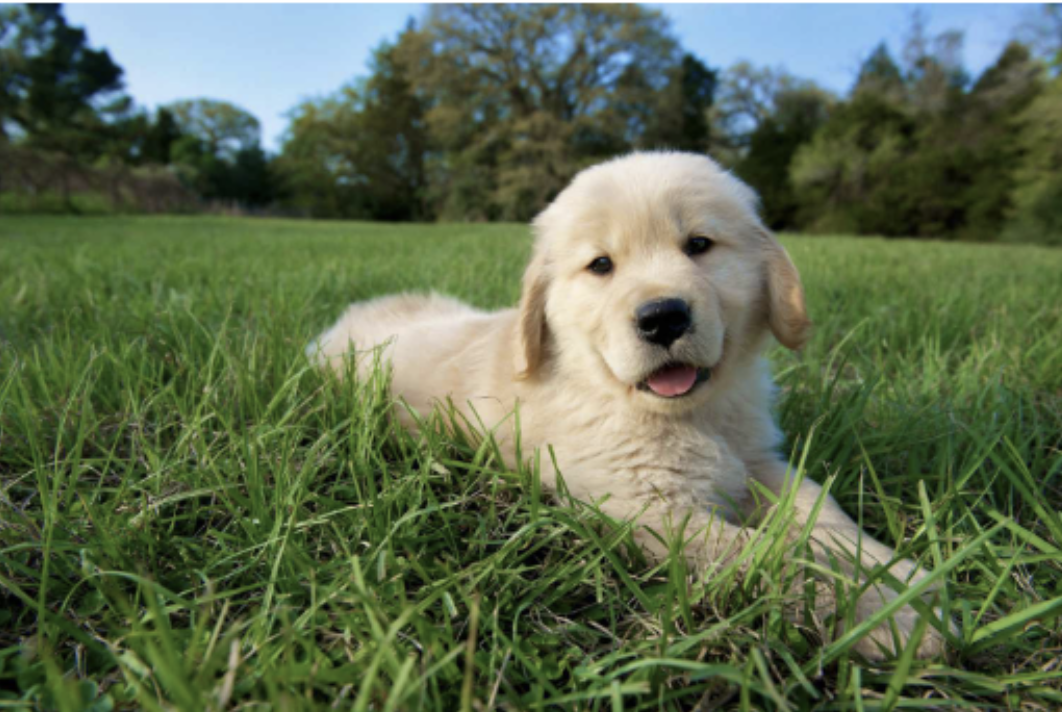
\includegraphics[width=7cm,clip]{/Users/jgooding/Documents/SMARTHEP/CHEP2023/CHEP2023/proceedings/figures/placeholder.png}
    \caption{Diagram demonstrating the real-time analysis approach to data processing.}
    \label{rta-diagram}       % Give a unique label
\end{figure*}



\subsection{Tools of RTA}
\label{rta-tools}
Online processing of data has been enabled by advances in computing over the past two decades, particularly in the areas of machine learning and hybrid architectures.

\subsubsection{Machine learning}
\label{machine-learning}
Central to the RTA approach is rapid decision making on complex data. Often such decision making is challenging to implement using classical selection cuts  \cite{albertsson-ml}.\par
Machine learning techniques can also be applied to pattern recognition and anomaly detection—tasks which cannot be realistically carried out on the scales of data presently being analysed.

\subsubsection{Hybrid architectures}
\label{hybrid-architectures}
Typical computational resources consist of Central Processing Units (CPUs), processors which are designed for general purpose computation, with large on-board memory and often multiple processing cores. Alternative architectures, such as those shown in Figure~\ref{architectures}, can be applied in conjunction or in place of CPU architectures to accelerate processing where the . \par
Field-programmable gate arrays (FPGAs) \cite{duarte-fpgas}. FPGAs are thus well-suited to bespoke, computationally light but highly parallelisable tasks, such as low-level trigger decisions.\par
Graphical Processing Units (GPUs) can also be employed to . \cite{vomBruch-gpus}
\begin{figure*}
    \centering
    % Use the relevant command for your figure-insertion program
    % to insert the figure file. See example above.
    % If not, use
    \vspace*{5cm}       % Give the correct figure height in cm
    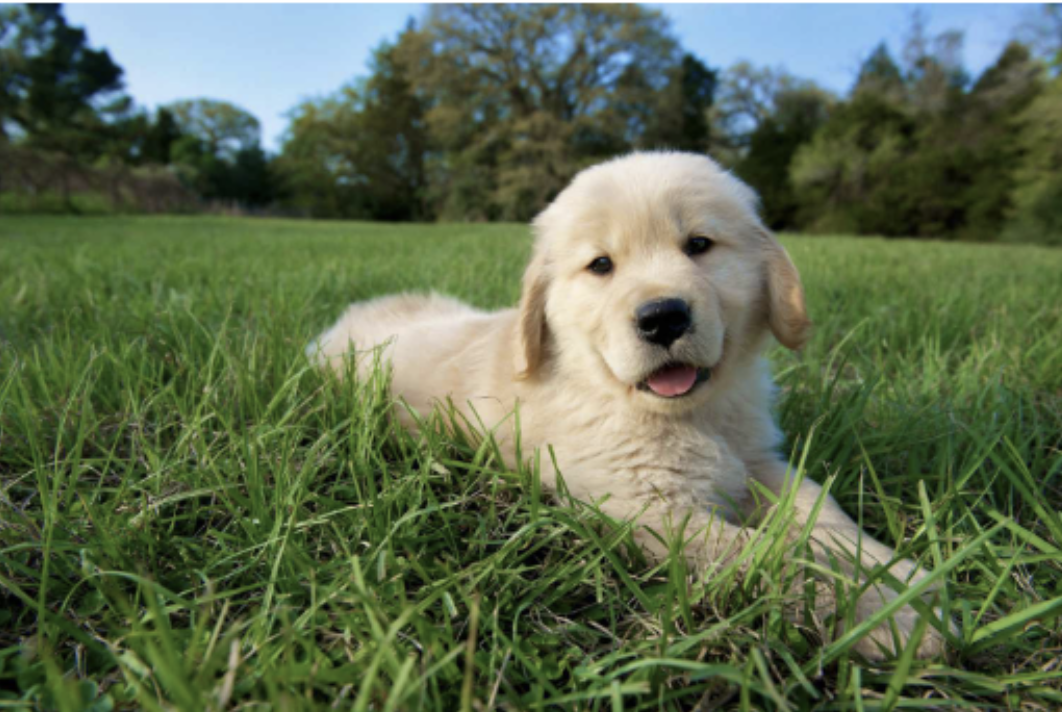
\includegraphics[width=7cm,clip]{/Users/jgooding/Documents/SMARTHEP/CHEP2023/CHEP2023/proceedings/figures/placeholder.png}
    \caption{Comparison of computing architectures.}
    \label{architectures}       % Give a unique label
\end{figure*}